\documentclass[10pt]{extarticle}

% Lingua e matematica
\usepackage[english]{babel}
\usepackage{amsmath,amssymb,amsthm}

% Grafica e tabelle
\usepackage{graphicx}
\usepackage{subcaption}
\usepackage{float}
\usepackage{booktabs}
\usepackage{multirow}
\usepackage{siunitx}
\usepackage{wrapfig}
%\usepackage[section]{placeins}  % mantiene i float dentro la SECTION
%\let\Oldsubsection\subsection   % estendo il comportamento anche alle SUBSECTION
%\renewcommand{\subsection}{\FloatBarrier\Oldsubsection}
\usepackage{placeins}


% Codice (opzionale)
\usepackage{listings}
\usepackage{xcolor}
\definecolor{codegreen}{rgb}{0,0.6,0}
\definecolor{codegray}{rgb}{0.5,0.5,0.5}
\definecolor{codepurple}{rgb}{0.58,0,0.82}
\definecolor{backcolour}{rgb}{0.98,0.98,0.98}
\lstdefinestyle{mystyle}{
  backgroundcolor=\color{backcolour},
  commentstyle=\color{codegreen},
  keywordstyle=\color{magenta},
  numberstyle=\tiny\color{codegray},
  stringstyle=\color{codepurple},
  basicstyle=\ttfamily\footnotesize,
  breaklines=true, keepspaces=true, numbers=none, tabsize=2
}
\lstset{style=mystyle}

% Margini
\usepackage[margin=0.6in]{geometry}
\usepackage{ragged2e}
\usepackage{enumitem}
%\usepackage[utf8]{inputenc} % per caratteri UTF-8 nei .tex e nel .bib
\usepackage[backend=biber,style=ieee,sorting=none,maxbibnames=99]{biblatex}
\ExecuteBibliographyOptions{doi=true,url=true,isbn=false}
\addbibresource{references.bib}
\usepackage{csquotes}       % consigliato da biblatex (evita warning e parse strani)
\usepackage{pifont}
\newcommand{\good}[1]{\textcolor{teal!70!black}{\ding{51}~#1}}



% Bibliografia (biblatex + biber)
\usepackage[backend=biber,style=ieee]{biblatex}
\addbibresource{references.bib}

% TOC: includi anche \paragraph e numerali
\setcounter{secnumdepth}{2}
\setcounter{tocdepth}{2}

% Hyperref (sempre *dopo* gli altri pacchetti)
\usepackage[colorlinks=true,linkcolor=blue,citecolor=teal,urlcolor=magenta]{hyperref}


\begin{document}

% Custom header without a separate titlepage
\noindent
\begin{minipage}{0.3\textwidth}
    
\includegraphics[width=1.3\linewidth]{Figures/polito_logo_2021_blu.jpg}
\end{minipage}
\hfill
\begin{minipage}{0.68\textwidth}
    \raggedleft
    {\LARGE \textbf{Politecnico di Torino}}\\[0.2cm]
    {\large Master's Degree in Mathematical Engineering}\\[0.7cm]
    {\large \textbf{Material for Thesis}}\\[0.2cm]
    {\large e-- Data Pre-processing Pipeline \\ Age Study}\\[0.7cm]
    \begin{tabular}{rl}
        Elisabetta Roviera & \texttt{s328422} \\
    \end{tabular}
\end{minipage}

\vspace{1cm}
\hrule
\vspace{0.5cm}

\tableofcontents

\vspace{0.5cm}
\hrule
\vspace{1cm}


% Main content begins here, on the same page
\justifying

\begin{abstract}
This document investigates the role of age-dependent DNA methylation in breast tissue by integrating epigenetic age modelling into the DNA methylation pre-processing pipeline. The analysis focuses on the estimation of DNA methylation age using the multi-tissue epigenetic clock proposed by Horvath and on the characterization of age-related methylation structure in normal and tumor-adjacent breast tissue.

Age-dependent methylation patterns are evaluated in light of their biological relevance to cancer susceptibility, following the framework proposed by Teschendorff et al. \cite{Teschendorff2010}, and are used to motivate age stratification into biologically meaningful bins. The study further assesses the impact of age as a confounding factor shaping global methylation variability and justifies its explicit control in downstream analyses.

The implementation is available at
\href{https://github.com/elisabettaroviera/THESIS/blob/main/01%20-%20Notebook/02%20-%20Data%20Pre-Processing/Age/02-age-dependent-dna-teschendorff.ipynb}{\texttt{02-age-dependent-dna-teschendorff.ipynb}}.
\end{abstract}


% ============================================================
% Epigenetic Age Estimation
% ============================================================

\section{Epigenetic Age Estimation}

\paragraph{Biological ageing and epigenetic clocks}
Chronological age represents the time elapsed since birth and provides only a coarse approximation of the biological processes underlying ageing. Individuals of the same chronological age may exhibit markedly different physiological states, disease susceptibility, and mortality risk, reflecting heterogeneity in biological ageing trajectories. For this reason, considerable effort has been devoted to the identification of molecular biomarkers capable of capturing ageing-related changes at the cellular and tissue level.

DNA methylation has emerged as one of the most robust molecular correlates of ageing. Age-associated methylation changes occur reproducibly at specific CpG sites across the genome and accumulate in a largely monotonic manner over time. Epigenetic clocks leverage this property by combining methylation levels at selected CpG sites into a predictive model that estimates an individual's \emph{biological age}, commonly referred to as DNA methylation age (DNAmAge). Such clocks have been shown to correlate strongly with chronological age while also capturing deviations associated with environmental exposures, disease states, and tissue-specific stressors \cite{Horvath2013,Zhang2019}.

\paragraph{DNA methylation age and age acceleration}
DNA methylation age is defined as the age predicted by an epigenetic clock from DNA methylation data. Unlike chronological age, DNAmAge reflects cumulative molecular alterations associated with ageing processes. The difference between DNAmAge and chronological age, often termed \emph{age acceleration}, is interpreted as an indicator of altered biological ageing: positive values suggest accelerated ageing, whereas negative values indicate decelerated ageing. Age acceleration has been associated with age-related diseases, cancer risk, and mortality across multiple studies, supporting its relevance as a biologically meaningful phenotype \cite{Horvath2013,Zhang2019}.

\paragraph{Epigenetic clocks: tissue-specific versus multi-tissue models}
Epigenetic clocks can be broadly classified into tissue-specific and multi-tissue models. Tissue-specific clocks, such as blood-based predictors, are optimized for high accuracy within a single biological context but may perform poorly when applied outside their training domain \cite{Varshavsky2023}. In contrast, multi-tissue clocks are explicitly designed to capture ageing-related methylation patterns that are conserved across diverse tissues and cell types, trading some degree of tissue-specific accuracy for robustness and generalizability \cite{Horvath2013,Zhang2019}. This distinction is critical when applying epigenetic clocks to solid tissues and pathological samples.

\paragraph{The Horvath multi-tissue epigenetic clock}
The epigenetic clock developed in \cite{Horvath2013} constitutes the first large-scale, multi-tissue DNA methylation age estimator. The model was trained on approximately 8,000 samples drawn from 82 publicly available datasets, spanning 51 distinct human tissues and cell types, including solid tissues and samples from diseased conditions. This broad and heterogeneous training set was deliberately chosen to ensure applicability across diverse biological contexts, rather than optimizing performance for a single tissue.

\paragraph{Mathematical formulation of the Horvath clock}
The Horvath clock is based on a penalized linear regression model using elastic net regularization. Starting from a candidate set of 21,369 CpG sites shared across Illumina 27k and 450k platforms, the elastic net procedure selects a subset of 353 CpG sites whose methylation levels jointly predict chronological age. For a given sample, DNAmAge is computed as a linear combination of the methylation beta values at these CpGs plus an intercept term,
\[
\text{DNAmAge} = \sum_{i=1}^{353} w_i \beta_i + b,
\]
where $\beta_i$ denotes the methylation level of the $i$-th CpG site and $w_i$ the corresponding regression coefficient. This formulation yields a continuous age estimate expressed in years. Despite its linear structure, the clock captures complex ageing-related patterns due to the joint contribution of CpGs distributed across multiple genomic regions.

\paragraph{Interpretation and applicability to breast tissue}
Although the Horvath clock was explicitly designed as a pan-tissue age predictor, its original publication reports that prediction accuracy varies substantially across tissues, with breast tissue ranking among the most challenging contexts for accurate age estimation \cite{Horvath2013}. Horvath attributes this reduced accuracy to several tissue-specific factors, including pronounced cellular heterogeneity, strong hormonal regulation, and extensive epigenetic remodeling associated with mammary gland development and differentiation. These characteristics introduce additional sources of variability in DNA methylation patterns that are not strictly age-driven, thereby reducing the signal-to-noise ratio of age-associated CpG changes.

Importantly, the Horvath clock was trained primarily on non-malignant tissues and cell types, and while it was evaluated across a wide range of biological contexts, it was not designed to provide accurate chronological age estimates in fully transformed tumor samples \cite{Horvath2013}. Malignant transformation is known to profoundly disrupt the epigenetic landscape through widespread DNA methylation alterations, including global hypomethylation and focal hypermethylation of regulatory regions. These cancer-associated changes decouple DNA methylation patterns from normal ageing trajectories, making the interpretation of DNAmAge in tumor tissue intrinsically problematic.

This limitation is supported by independent evidence showing that age-associated DNA methylation patterns are extensively altered in cancer. In particular, Teschendorff et al. \cite{Teschendorff2010} demonstrated that many CpG sites exhibiting age-dependent methylation in normal tissues undergo aberrant methylation changes in cancer, especially at genes suppressed in stem cells, highlighting a fundamental rewiring of epigenetic ageing signals during tumorigenesis. Similarly, subsequent work has shown that deviations between DNAmAge and chronological age in cancer samples reflect not only biological ageing but also tumor-specific epigenetic dysregulation \cite{Zhang2019}.

For these reasons, while the Horvath clock remains applicable and informative in non-malignant breast tissue—such as normal and adjacent samples—it must be applied with caution to tumor tissue. In malignant samples, widespread cancer-associated epigenetic alterations disrupt age-related DNA methylation patterns, thereby weakening the link between DNAmAge and physiological ageing. As a consequence, DNAmAge estimates in tumor tissue are more appropriately interpreted in a relative or comparative framework, rather than as absolute measures of biological age.
In the present study, DNAmAge estimation was therefore deliberately restricted to Normal and Adjacent breast tissue samples. Tumor samples were excluded from age estimation both for biological reasons, given the extensive epigenetic reprogramming induced by malignant transformation, and for methodological coherence with the primary objective of the study. 
% ============================================================
% Application to GSE225845
% ============================================================

\section{Application of the Horvath Clock to GSE225845 dataset}

\paragraph{Input data and preprocessing}
Epigenetic age estimation was performed on the GSE225845 dataset using DNA methylation beta values obtained after the complete preprocessing pipeline described in the previous sections. Briefly, preprocessing included probe-level technical filtering to remove cross-reactive probes, polymorphic CpGs, non-CpG probes, and probes mapping to sex chromosomes, in accordance with established best practices for Illumina methylation arrays. Missing values were handled conservatively, and beta values were subsequently normalized using the BMIQ algorithm to correct for Infinium Type I/II probe design bias. This normalization step is explicitly recommended in the original implementation of the Horvath clock and ensures compatibility with the assumptions underlying the model, while reducing technical sources of variation unrelated to biological ageing.

\paragraph{Sample selection}
Epigenetic age estimation was restricted to Normal and Tumor-Adjacent breast tissue samples (Normal + Adjacent). Tumor samples were deliberately excluded from DNAmAge estimation, as explained earlier. 

\paragraph{CpG coverage and imputation strategy}
The Horvath epigenetic clock requires methylation measurements for 353 CpG sites selected from a candidate set of 21,369 CpGs shared across Illumina 27k and 450k platforms. In the GSE225845 dataset, generated using the Illumina EPIC (850k) array, 316 of the required CpGs were directly available, while 37 CpGs were missing due to platform differences. Missing CpGs were imputed following the original procedure described in the Supplementary Methods, using platform-specific reference values (goldstandard or goldstandard2) provided in the official supplementary files when available, and a conservative default value of $\beta = 0.5$ otherwise \cite{Horvath2013}. This strategy ensures maximal consistency with the original model specification. After imputation, a complete set of 353 CpGs was obtained for each sample, enabling uniform application of the clock across all individuals.

\paragraph{Computation of DNAmAge and downstream metrics}
For each sample, DNAmAge was computed using the published regression coefficients and intercept of the Horvath model, as implemented in the original reference scripts. Chronological age at surgery was used as the reference age variable. Model performance was subsequently evaluated using standard accuracy metrics, including mean absolute error (MAE), root mean squared error (RMSE), Pearson correlation coefficient ($R$), coefficient of determination ($R^2$), and mean absolute percentage error (MAPE). In addition, age acceleration was defined as the signed difference between DNAmAge and chronological age and analyzed both globally and stratified by tissue group to assess tissue-specific ageing patterns.

% ============================================================
% Results
% ============================================================
\subsection{Results}

\paragraph{Global performance of epigenetic age estimation}
Epigenetic age estimation was successfully performed on all Normal and Tumor-Adjacent samples of the GSE225845 dataset ($n = 253$). Chronological age is treated as ground truth, while DNAmAge is used as a proxy to quantify epigenetic drift. Overall, DNAmAge exhibited a moderate-to-strong linear association with chronological age, indicating that the clock captures a substantial component of age-related methylation variability in breast tissue. A summary of global performance metrics is reported in Table~\ref{tab:horvath_global}. The observed accuracy is consistent with previous applications of the Horvath clock to tissue types that were not explicitly optimized during model training \cite{Horvath2013}.

\begin{table}[t]
\centering
\caption{Global performance of the Horvath epigenetic clock on GSE225845 (Normal + Adjacent samples).}
\label{tab:horvath_global}
\begin{tabular}{l c}
\toprule
Metric & Value \\
\midrule
Number of samples & 253 \\
MAE (years) & 9.989 \\
RMSE (years) & 11.691 \\
Pearson correlation ($R$) & 0.770 \\
Coefficient of determination ($R^2$) & 0.593 \\
MAPE (\%) & 22.735 \\
\bottomrule
\end{tabular}
\end{table}

\paragraph{Performance stratified by tissue group}
Stratification by tissue type revealed distinct behaviors between Normal and Tumor-Adjacent samples. As summarized in Table~\ref{tab:horvath_by_tissue}, Normal tissues exhibited a higher estimation error than Adjacent tissues, while maintaining a comparable correlation with chronological age. This indicates that, despite increased dispersion, DNAmAge preserves a consistent linear relationship with age across tissue contexts. The improved performance observed in Adjacent samples may reflect more homogeneous epigenetic alterations shared across samples, potentially associated with common environmental exposures or early field effects.

\begin{table}[t]
\centering
\caption{Performance of the Horvath epigenetic clock stratified by tissue group.}
\label{tab:horvath_by_tissue}
\begin{tabular}{l c c c c c c}
\toprule
Tissue & N & MAE (years) & RMSE (years) & $R$ & $R^2$ & MAPE (\%) \\
\midrule
Normal & 113 & 11.6 & 12.6 & 0.703 & 0.494 & 29.1 \\
Adjacent & 140 & 8.71 & 10.9 & 0.715 & 0.511 & 17.6 \\
\bottomrule
\end{tabular}
\end{table}

\paragraph{Age acceleration patterns}
Age acceleration was defined as the signed difference between DNAmAge and chronological age. At the global level, samples displayed a pronounced positive age acceleration, with a mean value of +7.57 years and a median of +9.10 years, indicating that breast tissue in this cohort is epigenetically older than expected based on chronological age alone. Tissue-specific analysis revealed markedly different patterns: Normal samples showed strong age acceleration (mean $\approx$ +10.9 years), whereas Adjacent samples exhibited a more moderate but more heterogeneous acceleration (mean $\approx$ +4.9 years). This distribution suggests that a subset of clinically normal tissues already displays substantial epigenetic ageing.

\paragraph{Visualization of age effects and methylation structure}
Figure~\ref{fig:age_and_pca} illustrates how chronological age and epigenetic age jointly shape the global DNA methylation structure. 
The boxplots provide a descriptive overview of cohort composition, showing systematic differences in both age at surgery and Horvath DNAmAge between Normal and Tumor-Adjacent tissues, and indicating the presence of substantial epigenetic age acceleration already in non-malignant samples.
Principal component analysis performed on raw methylation data reveals that age-related variables contribute structured variance to the methylome: while the association between the first principal component and chronological age is weak (corr(PC1, age) = $-0.03$), a more pronounced relationship emerges with DNAmAge (corr(PC1, DNAmAge) = $0.17$), suggesting that epigenetic age captures biologically meaningful variation beyond chronological time alone.
After explicit removal of age-related effects, these associations are effectively eliminated (corr(PC1, age) = $0.00$; corr(PC1, DNAmAge) = $0.00$), demonstrating that age acts as a confounding factor in global methylation patterns and that age residualization successfully removes this source of structure.
Together, these results indicate that epigenetic age captures organized component of methylation variability in breast tissue, consistent with the framework proposed by Teschendorff et al.~\cite{Teschendorff2010}, whereby age-dependent DNA methylation changes at genes suppressed in stem cells constitute a hallmark of cancer and may predispose tissue to malignant transformation.
The more moderate yet heterogeneous epigenetic age acceleration observed in Tumor-Adjacent tissue suggests an intermediate epigenetic state, compatible with early field cancerization rather than fully established malignant reprogramming.

\begin{figure}[htbp]
    \centering

    % -------------------- ROW 1 --------------------
    \begin{subfigure}[t]{0.30\textwidth}
        \centering
        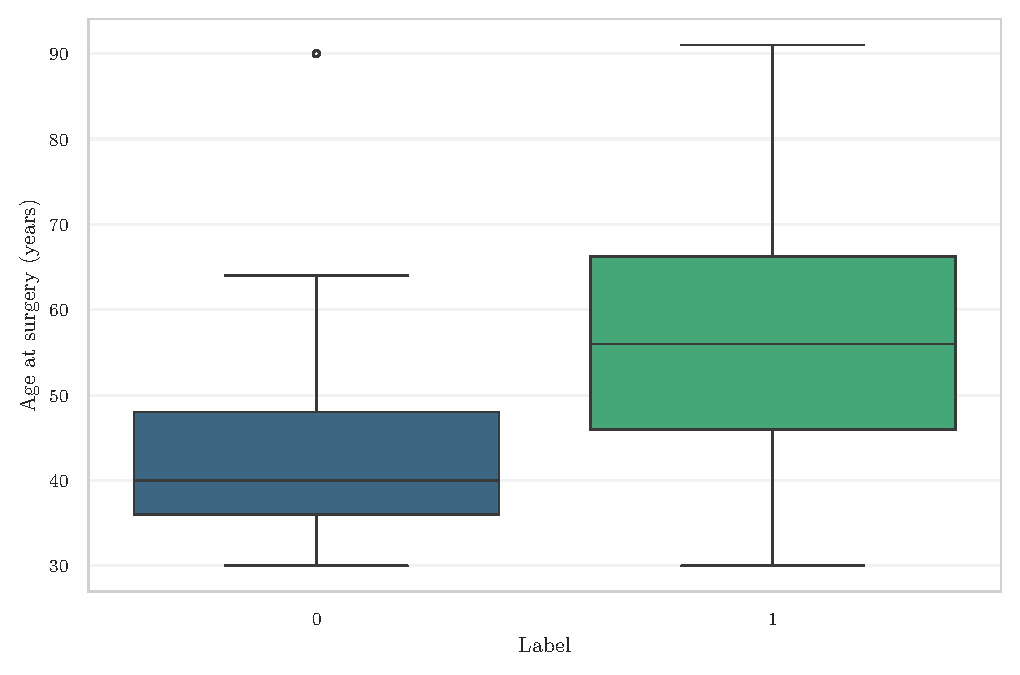
\includegraphics[width=\textwidth]{Figures/age_by_label_1.pdf}
        \caption{Chronological age at surgery by tissue group.}
        \label{fig:age_and_pca:age_true}
    \end{subfigure}
    \hfill
    \begin{subfigure}[t]{0.30\textwidth}
        \centering
        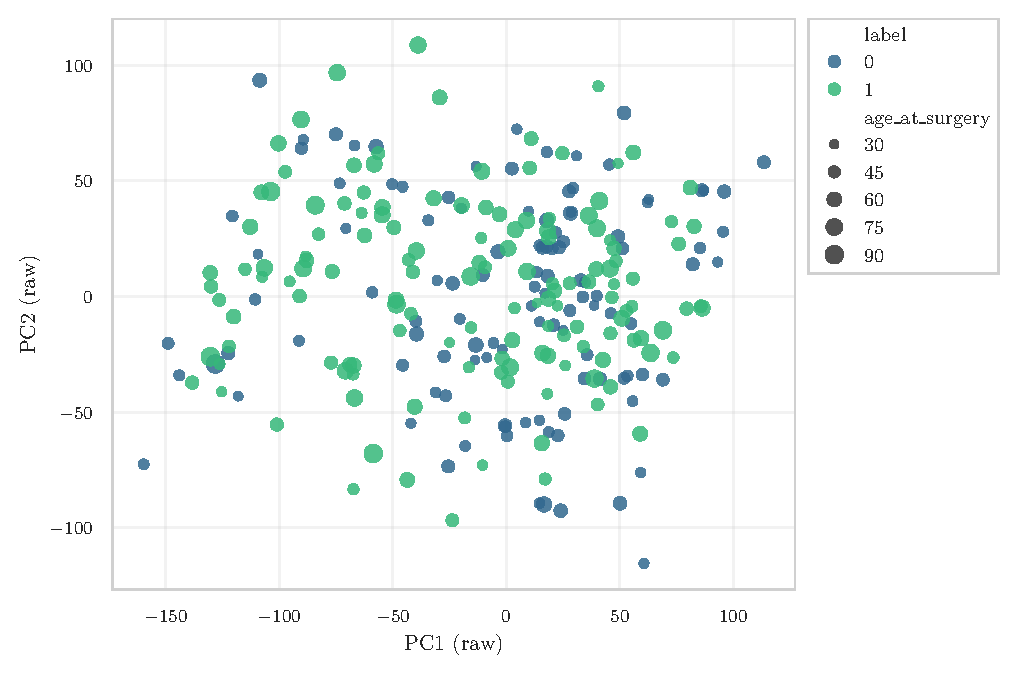
\includegraphics[width=\textwidth]{Figures/pca_raw_1.pdf}
        \caption{Raw methylation PCA (fit on Normal), colored by age.}
        \label{fig:age_and_pca:pca_raw_age}
    \end{subfigure}
    \hfill
    \begin{subfigure}[t]{0.30\textwidth}
        \centering
        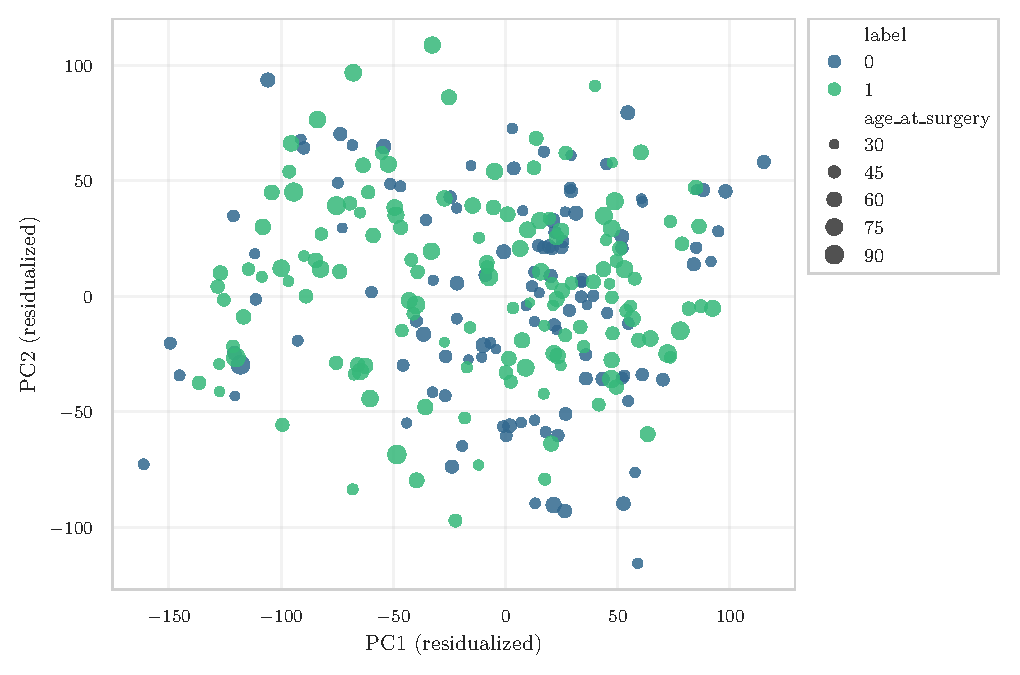
\includegraphics[width=\textwidth]{Figures/pca_residual_1.pdf}
        \caption{Residualized PCA after removal of age effects.}
        \label{fig:age_and_pca:pca_resid_age}
    \end{subfigure}

    \vspace{0.6em}

    % -------------------- ROW 2 --------------------
    \begin{subfigure}[t]{0.30\textwidth}
        \centering
        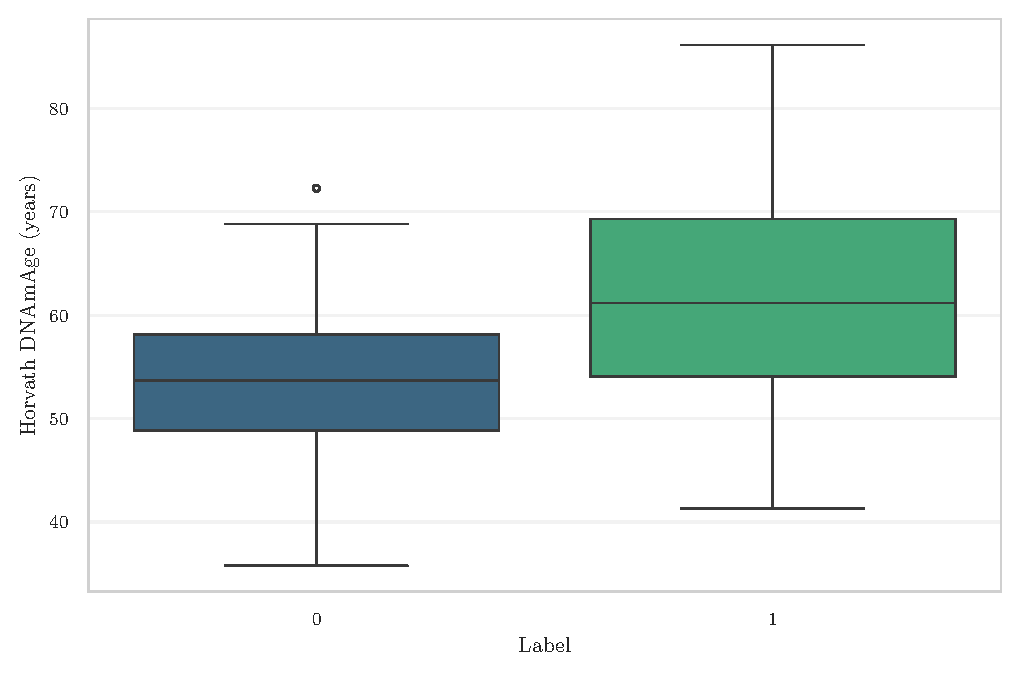
\includegraphics[width=\textwidth]{Figures/age_by_label_2.pdf}
        \caption{Horvath DNAmAge by tissue group.}
        \label{fig:age_and_pca:dnamage_by_label}
    \end{subfigure}
    \hfill
    \begin{subfigure}[t]{0.30\textwidth}
        \centering
        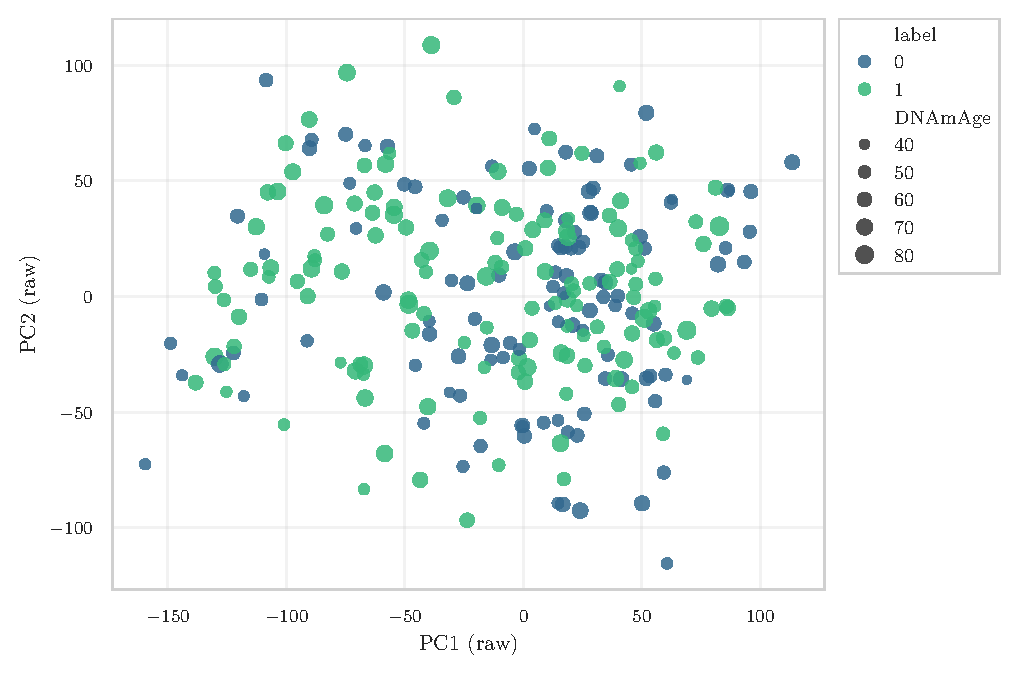
\includegraphics[width=\textwidth]{Figures/pca_raw_2.pdf}
        \caption{Raw methylation PCA (fit on Normal), colored by DNAmAge.}
        \label{fig:age_and_pca:pca_raw_dnamage}
    \end{subfigure}
    \hfill
    \begin{subfigure}[t]{0.30\textwidth}
        \centering
        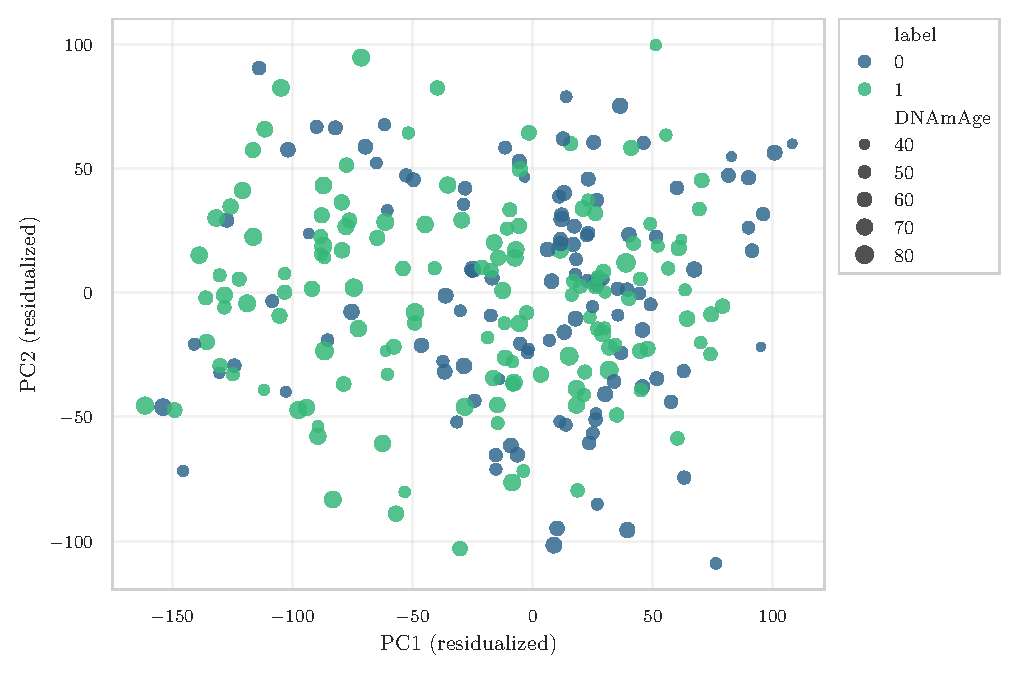
\includegraphics[width=\textwidth]{Figures/pca_residual_2.pdf}
        \caption{Residualized PCA after removal of age-related structure.}
        \label{fig:age_and_pca:pca_resid_dnamage}
    \end{subfigure}

    \caption{\textbf{Age-driven structure of the breast tissue methylome.}
    Boxplots summarize cohort composition in terms of chronological age and epigenetic age across tissue groups.
    PCA embeddings computed on raw methylation data reveal that age-related variables contribute structured variance to the methylome, while residualized PCA demonstrates that regressing out age effectively removes this confounding component.
    Together, the panels motivate age adjustment in downstream analyses.}
    \label{fig:age_and_pca}
\end{figure}

% ============================================================
% Age Binning Strategy
% ============================================================
\subsection{Age Binning Strategy}

\paragraph{Biological motivation for age discretization}
Beyond its continuous effect on DNA methylation, age marks distinct biological phases in breast tissue that are associated with major hormonal and physiological transitions. In particular, the menopausal transition represents a well-defined biological breakpoint characterized by profound changes in estrogen exposure, tissue composition, and cancer risk. Large-scale epidemiological studies have shown that the median age at natural menopause in Western populations lies between 50 and 52 years, with relatively limited inter-individual variability \cite{Gold2013}. This biological landmark provides a clinically and physiologically grounded justification for separating pre-/peri-menopausal and post-menopausal age groups when studying breast tissue biology.

In this context, discretizing age into biologically motivated bins allows the analysis to reflect non-linear transitions in tissue state rather than assuming a uniform, linear effect of age across the entire lifespan. This approach is consistent with clinical evidence indicating that breast cancer arising before and after menopause differs in incidence, molecular characteristics, and prognosis \cite{Azim2012}.

\paragraph{Definition and interpretation of age bins}
Age bins were therefore defined to capture distinct phases of breast tissue aging associated with different hormonal environments: young ($\leq 40$ years), peri-menopausal (41--52 years), post-menopausal (53--64 years), and elderly ($\geq 65$ years). These intervals align with established clinical and epidemiological definitions of reproductive aging and are intended to enhance the biological interpretability of downstream stratified analyses. 

Importantly, age binning was deliberately introduced to mitigate the impact of estimation error inherent to continuous epigenetic age prediction and to shift the analytical focus from precise age reconstruction to biologically meaningful age stratification. Given the known uncertainty of epigenetic age estimates in breast tissue, particularly in non-blood contexts, discretizing age into clinically and biologically motivated bins allows a more robust interpretation of results by reducing sensitivity to small prediction errors near decision boundaries.
Moreover, the primary objective of this study is not to recover an exact biological age, but to correctly assign samples to age ranges that are known to be associated with distinct breast cancer biology. Substantial evidence indicates that breast cancer arising in younger, peri-menopausal, and post-menopausal women differs in terms of tumor subtype distribution, molecular characteristics, and clinical behavior \cite{Azim2012}. From this perspective, correct bin assignment is more relevant than precise age estimation, as it aligns the epigenetic analysis with biologically distinct disease contexts rather than with a continuous chronological scale.

\paragraph{Distribution of samples across age bins}
After validating the behavior of the Horvath epigenetic clock on the GSE225845 dataset, for which chronological age at surgery is available, the same clock was subsequently applied to the remaining datasets. For these cohorts, epigenetic age was estimated and samples were assigned to biologically motivated age bins, enabling a unified stratification framework across all datasets.

Figure~\ref{fig:age_bin_distribution} reports the distribution of samples across age bins in the three analyzed cohorts. Although the datasets differ in cohort composition, sample size, and experimental design, a consistent pattern emerges: the majority of samples fall within peri- and post-menopausal age ranges. This reflects both the epidemiology of breast tissue sampling in clinical studies and the age distribution at which breast cancer and related tissue alterations are most frequently investigated. Younger samples are comparatively underrepresented, particularly in GSE225845, whereas elderly samples are present in all cohorts but with variable prevalence.

Importantly, this heterogeneous yet comparable distribution across datasets supports the use of age bins as a robust stratification variable. Age binning allows meaningful cross-dataset comparisons even when exact chronological age information is unavailable, while preserving biologically relevant distinctions associated with different phases of breast tissue ageing and disease risk.

\begin{figure}[t]
    \centering
    \begin{subfigure}[t]{0.32\textwidth}
        \centering
        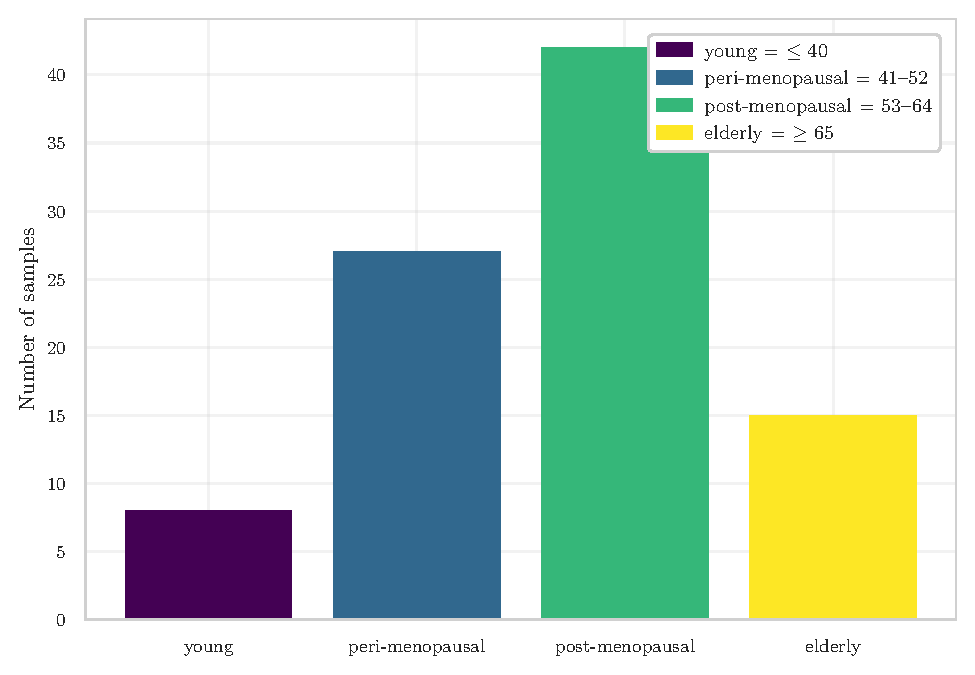
\includegraphics[width=\textwidth]{Figures/GSE69914_bin_counts.pdf}
        \caption{GSE69914}
        \label{fig:age_bins:gse69914}
    \end{subfigure}
    \hfill
    \begin{subfigure}[t]{0.32\textwidth}
        \centering
        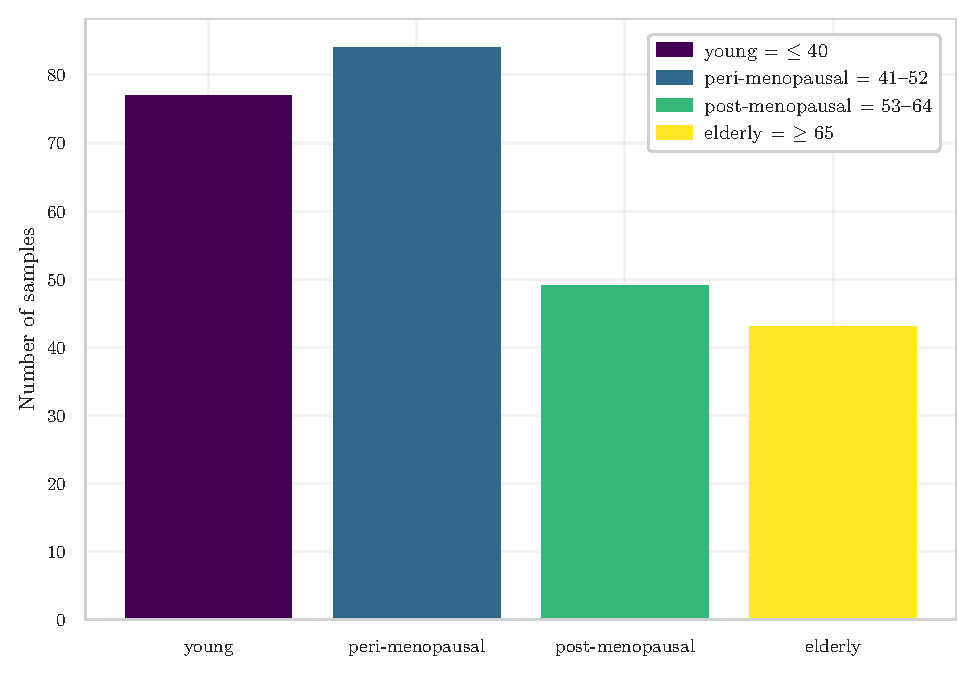
\includegraphics[width=\textwidth]{Figures/GSE225845_bin_counts.pdf}
        \caption{GSE225845}
        \label{fig:age_bins:gse225845}
    \end{subfigure}
    \hfill
    \begin{subfigure}[t]{0.32\textwidth}
        \centering
        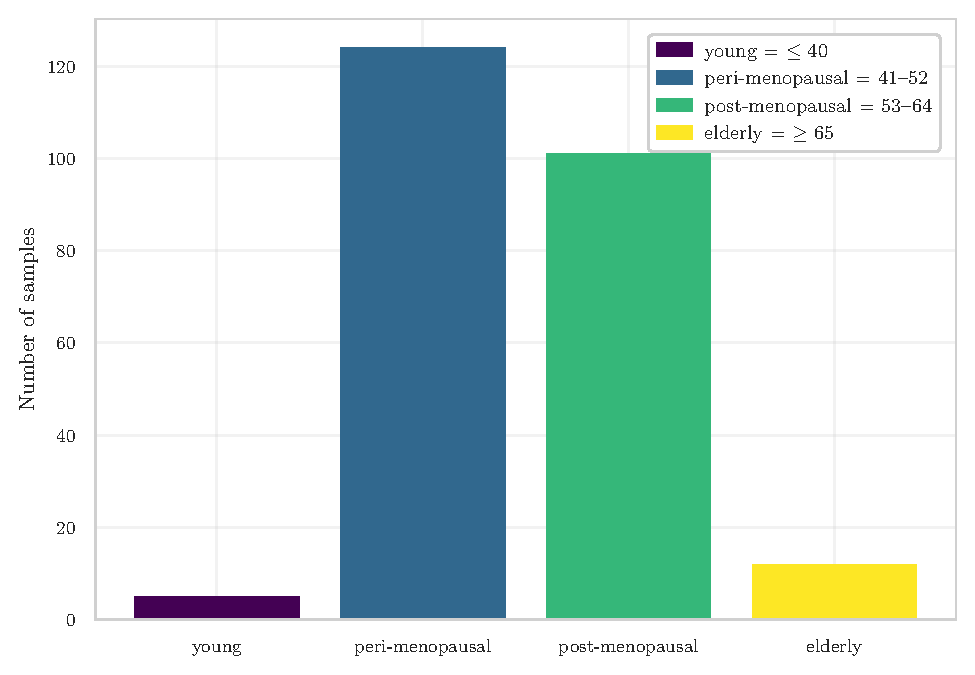
\includegraphics[width=\textwidth]{Figures/GSE287331_bin_counts.pdf}
        \caption{GSE287331}
        \label{fig:age_bins:gse287331}
    \end{subfigure}

    \caption{\textbf{Distribution of samples across epigenetic age bins in the analyzed datasets.}
    Age bins are defined as: young ($\leq 40$ years), peri-menopausal (41--52 years), post-menopausal (53--64 years), and elderly ($\geq 65$ years).
    Bars report the number of samples assigned to each age bin in each dataset.
    The predominance of peri- and post-menopausal samples reflects the clinical age distribution of breast tissue cohorts and motivates age-stratified analyses.}
    \label{fig:age_bin_distribution}
\end{figure}

% ============================================================
% Downstream analysis constraints
% ============================================================

\section{Methodological constraints for downstream analyses}

Following the epigenetic age analysis, Horvath DNAmAge was estimated for all datasets and subsequently discretized into biologically motivated age bins. This step provides a unified and robust age stratification framework across cohorts, including datasets lacking chronological age information, and enables consistent downstream comparisons grounded in biologically meaningful age groups.

To prevent information leakage and circularity, all CpG sites used by the Horvath epigenetic clock were explicitly excluded from the CpG set employed in subsequent analyses. By removing clock-associated CpGs, age-related signals captured during age modelling are prevented from trivially reappearing in downstream feature selection and differential methylation analyses.

Together, these steps establish a clear methodological separation between age modelling and downstream epigenomic investigation, ensuring that subsequent analyses focus on methylation patterns beyond those directly driving epigenetic age estimation.








\printbibliography
\end{document}
